\documentclass[12pt,a4paper]{article}

\usepackage[utf8]{inputenc}
\usepackage[T1]{fontenc}
\usepackage{amsmath,amssymb,amsthm}
\usepackage{graphicx}
\usepackage{float}
\usepackage[margin=2.5cm]{geometry}
\usepackage{hyperref}
\usepackage{xcolor}
\usepackage{booktabs}
\usepackage{natbib}
\usepackage{tikz}
\usetikzlibrary{arrows.meta,decorations.pathmorphing,calc}

\newtheorem{theorem}{Theorem}
\newtheorem{corollary}[theorem]{Corollary}
\newtheorem{proposition}[theorem]{Proposition}
\newtheorem{definition}{Definition}
\newtheorem{remark}{Remark}

\title{\textbf{Combinatorial Shadow: How Dimensional Mismatch\\Generates Apparent Complexity,\\with Applications to Social Hierarchy}}

\author{Ian Todd\\
Sydney Medical School\\
University of Sydney\\
Sydney, NSW, Australia\\
\texttt{itod2305@uni.sydney.edu.au}}

\date{\today}

\begin{document}

\maketitle

\begin{abstract}
We argue that the apparent combinatorial complexity experienced by a low-dimensional observer encountering a high-dimensional system is governed by the dimensional gap between them.
For systems whose attractor has box-counting dimension $\delta$, the number of states compatible with any single $d$-dimensional observation scales asymptotically as $\varepsilon^{-(\delta - d)}$---polynomial in resolution but exponential in the dimensional gap.
For systems characterised instead by a participation ratio $D_{\mathrm{eff}}$, we propose $D_{\mathrm{eff}} - d$ as a heuristic proxy for the same scaling, supported by simulation.
This reframes combinatorial explosion as a property of projection, not of the system itself.
We show via the chain rule for entropy that, when the total system satisfies $\Delta S_D \geq 0$, apparent negentropy in observed dimensions ($\Delta S_d < 0$) is necessarily balanced by entropy increase in the hidden conditional distribution ($\Delta S_{D-d|d} \geq |\Delta S_d|$), providing a bookkeeping identity that clarifies---though does not by itself resolve---the thermodynamic puzzle of Maxwell's demon.
We apply these ideas to social hierarchy formation, building agent-based models inspired by Bonabeau's (1996) emergent dominance framework with tunable kernel dimensionality.
Simulations confirm that hierarchy complexity tracks kernel dimensionality, that defence mechanisms function as dimensionality caps, and that sufficiently strong suppression dominates the social structure.
We close with a speculative conjecture connecting these results to consciousness and psychedelic phenomenology.
\end{abstract}

\medskip
\noindent\fbox{\parbox{\dimexpr\linewidth-2\fboxsep-2\fboxrule}{%
\textbf{On ``dimensionality.''} Throughout this paper we use \emph{dimensionality} in the \textbf{ML/complex-systems sense}: the effective/intrinsic degrees of freedom of accessible dynamics (e.g., participation ratio or effective rank of covariance/response spectra, or measure of the coherently accessible region)---\textbf{not} geometric embedding dimension. Measurement is dimensional collapse.}}
\medskip

%% ============================================================
%% PART I: THE GEOMETRIC RESULT
%% ============================================================

\section*{Part I: The Geometric Result}

\section{Introduction}

Combinatorial explosion is treated, almost universally, as a property of the system under study.
A chess game has $\sim 10^{120}$ possible games; a proteome has $20^{300}$ possible sequences; a social group of $N$ agents admits $2^{N(N-1)/2}$ possible interaction graphs.
The standard response is to seek algorithms, heuristics, or approximations that tame the explosion from within.

We argue this framing is backwards.
Combinatorial explosion is not a property of the system.
It is a property of the \emph{projection}---the dimensional mismatch between the system and its observer.

The intuition is simple.
A smooth trajectory in $D$ dimensions, when projected to $d < D$ dimensions, can appear to branch, cross itself, and generate apparent discontinuities.
The observer, unable to resolve the missing $D - d$ dimensions, interprets smooth high-dimensional flow as combinatorial complexity.
The explosion is in the shadow, not the thing.

This paper makes this intuition precise.
We show that the number of system states compatible with any single low-dimensional observation grows exponentially in the dimensional gap $\delta - d$, where $\delta$ is the attractor's box-counting dimension (Theorem~\ref{thm:main}).
We derive a conditional entropy decomposition showing that apparent negentropy in observed dimensions is balanced by entropy increase in hidden dimensions (Corollary~\ref{cor:compensation}), clarifying the dimensional bookkeeping behind Maxwell's demon.

We then apply these ideas to social hierarchy.
Bonabeau et al.~\citeyearpar{bonabeau1996} showed that dominance hierarchies emerge spontaneously from pairwise interactions between identical agents---agents with a one-dimensional state variable.
We build agent-based models with $D$-dimensional state vectors and show that hierarchy complexity tracks kernel dimensionality: a low-dimensional kernel produces a clean linear hierarchy; a high-dimensional kernel produces a complex, multi-axis social structure.
Defence mechanisms function as dimensionality caps, and sufficiently strong suppression determines the society's effective dimensionality.

We close with a speculative conjecture connecting these results to consciousness.

\section{Preliminaries}
\label{sec:prelim}

\begin{definition}[Box-counting dimension]
For a compact set $A \subset \mathbb{R}^D$, the \emph{box-counting (Minkowski) dimension} is
\begin{equation}
\dim_B(A) = \lim_{\varepsilon \to 0} \frac{\log N_\varepsilon(A)}{\log(1/\varepsilon)}
\end{equation}
where $N_\varepsilon(A)$ is the minimum number of $\varepsilon$-cubes needed to cover $A$.
This is the geometric quantity that controls fiber complexity under projection.
\end{definition}

\begin{definition}[Effective dimensionality]
For a system with state covariance matrix $\Sigma$ having eigenvalues $\lambda_1 \geq \lambda_2 \geq \cdots \geq \lambda_N \geq 0$, the \emph{effective dimensionality} is the participation ratio:
\begin{equation}
D_{\mathrm{eff}} = \frac{\left(\sum_{i=1}^{N} \lambda_i\right)^2}{\sum_{i=1}^{N} \lambda_i^2}
\label{eq:deff}
\end{equation}
This is a distributional measure: it equals $N$ when all eigenvalues are identical and approaches $1$ when variance concentrates in a single mode.
$D_{\mathrm{eff}}$ is not in general equal to $\dim_B(A)$, but for many attractors it provides a useful proxy.
We use $\dim_B$ in the rigorous theorem and $D_{\mathrm{eff}}$ as a practical estimator in simulations.
\end{definition}

\begin{definition}[Generic linear projection]
A \emph{generic linear projection} $P: \mathbb{R}^D \to \mathbb{R}^d$ is a surjective linear map whose kernel $\ker(P)$ is a $(D-d)$-dimensional subspace of $\mathbb{R}^D$ in general position with respect to the attractor $A$.
Concretely, for almost every choice of $d$ rows from a standard Gaussian matrix, the resulting projection is generic.
\end{definition}

\begin{definition}[Fiber]
For a projection $P$ and a point $y \in P(A)$, the \emph{fiber} over $y$ is
\begin{equation}
F(y) = P^{-1}(y) \cap A = \{x \in A : P(x) = y\}.
\end{equation}
This is the set of all system states compatible with the observation $y$.
\end{definition}

The Johnson-Lindenstrauss lemma \citep{johnson1984} guarantees that pairwise distances are approximately preserved under random projection from $\mathbb{R}^D$ to $\mathbb{R}^d$ with $d = O(\log n / \varepsilon^2)$ for $n$ points and distortion $\varepsilon$.
This is the good news about projection: metric structure survives.
The bad news is that \emph{topology} does not.
Distinct points in $A$ that are far apart in $\mathbb{R}^D$ can map to nearby or identical points in $\mathbb{R}^d$.
The fiber $F(y)$ captures exactly this degeneracy.


\section{Main Result: Projection Complexity Bound}
\label{sec:main}

\begin{theorem}[Projection Complexity Scaling]
\label{thm:main}
Let $A \subset \mathbb{R}^D$ be a compact attractor with box-counting dimension $\dim_B(A) = \delta$, and let $P: \mathbb{R}^D \to \mathbb{R}^d$ be a generic linear projection with $d < \delta$.
Then for a generic observation $y \in P(A)$, the number of $\varepsilon$-distinguishable states in the fiber $F(y) = P^{-1}(y) \cap A$ satisfies
\begin{equation}
\liminf_{\varepsilon \to 0} \frac{\log N_\varepsilon(y)}{\log(1/\varepsilon)} \geq \delta - d
\label{eq:main}
\end{equation}
That is, $N_\varepsilon(y)$ grows at least as fast as $\varepsilon^{-(\delta - d)}$ as $\varepsilon \to 0$.
\end{theorem}

\begin{proof}[Proof sketch]
The fiber $F(y) = P^{-1}(y) \cap A$ is the intersection of $A$ with a $(D-d)$-dimensional affine subspace.
For a generic projection and a generic point $y$, the box-counting dimension of $F(y)$ is $\max(0, \delta - d)$ by the dimension formula for generic linear sections (Mattila, \emph{Geometry of Sets and Measures}, Theorem~10.11; the result requires genericity to avoid pathological alignments).
The scaling~\eqref{eq:main} then follows from the definition of box-counting dimension applied to the fiber.
\end{proof}

\begin{remark}
The scaling is polynomial in $1/\varepsilon$ but \textbf{exponential in the dimensional gap} $\delta - d$.
At any fixed resolution, doubling the gap squares the number of compatible states.
The ``combinatorial explosion'' the observer experiences is governed by this gap.
\end{remark}

\begin{remark}[Participation ratio as heuristic proxy]
\label{rem:deff}
In practice, $\dim_B(A)$ is difficult to estimate from data.
The participation ratio $D_{\mathrm{eff}}$ (Eq.~\ref{eq:deff}) provides a computationally tractable proxy.
For systems whose variance is approximately uniformly spread across $\delta$ modes, $D_{\mathrm{eff}} \approx \delta$.
However, $D_{\mathrm{eff}}$ is a distributional quantity that can be non-integer and does not in general equal $\dim_B(A)$.
We use $D_{\mathrm{eff}}$ in the simulations below as an estimator, not as a substitute for the geometric dimension in Theorem~\ref{thm:main}.
\end{remark}

\begin{corollary}[Information deficit]
\label{cor:info}
The information required to specify which fiber element produced the observation $y$ scales as
\begin{equation}
I_{\mathrm{deficit}}(y) = \log_2 N_\varepsilon(y) \gtrsim (\delta - d) \cdot \log_2(1/\varepsilon)
\label{eq:info_deficit}
\end{equation}
asymptotically in $\varepsilon$.
This grows linearly in the dimensional gap.
For a system with $\delta = 20$ observed at $d = 3$ and $\varepsilon = 0.01$, the deficit is of order $17 \times 6.6 \approx 113$ bits per observation.
\end{corollary}


\section{Entropy Decomposition and Maxwell's Demon}
\label{sec:entropy}

The projection complexity bound has a direct thermodynamic interpretation.

\begin{theorem}[Conditional Entropy Decomposition]
\label{thm:entropy}
Let $X(t) \in \mathbb{R}^D$ be a stochastic process with time-dependent covariance $\Sigma(t)$, and let $P: \mathbb{R}^D \to \mathbb{R}^d$ be a linear projection.
Decompose the state as $X = (X_{\mathrm{obs}}, X_{\mathrm{hid}})$ where $X_{\mathrm{obs}} = PX \in \mathbb{R}^d$ and $X_{\mathrm{hid}}$ captures the remaining $D - d$ components.
Then by the chain rule for differential entropy:
\begin{equation}
S_D(t) = S_d(t) + S_{D-d \mid d}(t)
\label{eq:entropy_decomp}
\end{equation}
where $S_{D-d \mid d} = h(X_{\mathrm{hid}} | X_{\mathrm{obs}})$ is the conditional entropy of the hidden dimensions given the observed state.
This is an identity, not an approximation.
\end{theorem}

\begin{proof}
This is simply the chain rule: $h(X) = h(X_{\mathrm{obs}}) + h(X_{\mathrm{hid}} | X_{\mathrm{obs}})$.
\end{proof}

\begin{corollary}[Conditional compensation]
\label{cor:compensation}
If the full system satisfies $\Delta S_D \geq 0$ (second law), then whenever $\Delta S_d < 0$:
\begin{equation}
\Delta S_{D-d \mid d} \geq |\Delta S_d|
\label{eq:demon}
\end{equation}
The conditional entropy of the hidden dimensions must increase by at least as much as the observed entropy decreases.
\end{corollary}

\begin{proof}
From Eq.~\eqref{eq:entropy_decomp}: $\Delta S_D = \Delta S_d + \Delta S_{D-d \mid d}$.
If $\Delta S_D \geq 0$ and $\Delta S_d < 0$, then $\Delta S_{D-d \mid d} = \Delta S_D - \Delta S_d \geq |\Delta S_d|$.
\end{proof}

\medskip
\noindent\fbox{\parbox{\dimexpr\linewidth-2\fboxsep-2\fboxrule}{%
\textbf{Maxwell's Demon as Dimensional Bookkeeping.}
Consider a $d$-dimensional observer watching a $D$-dimensional system.
When the system performs coherent work visible to the observer ($\Delta S_d < 0$), the observer perceives an apparent entropy decrease.
But by Corollary~\ref{cor:compensation}, the conditional entropy of the hidden dimensions must increase by at least $|\Delta S_d|$.
This is a bookkeeping identity, not a thermodynamic mechanism: it tells us \emph{where to look} for the compensating entropy, not \emph{how} the compensation occurs.
The classical resolutions via Landauer's principle and Szilard's engine identify the mechanism; the dimensional decomposition identifies the geometry.}}

\subsection{Gaussian illustration}

For concreteness, consider a $D$-dimensional Gaussian process with covariance $\Sigma(t)$.
The differential entropy is
\begin{equation}
S_D(t) = \frac{1}{2}\log\det\!\left(2\pi e\,\Sigma(t)\right) = \frac{D}{2}\log(2\pi e) + \frac{1}{2}\sum_{i=1}^D \log \lambda_i(t)
\end{equation}
where $\lambda_i(t)$ are the eigenvalues of $\Sigma(t)$.
The projected entropy for an orthogonal projection onto the first $d$ coordinates is
\begin{equation}
S_d(t) = \frac{d}{2}\log(2\pi e) + \frac{1}{2}\sum_{i=1}^d \log \lambda^{(d)}_i(t)
\end{equation}
where $\lambda^{(d)}_i$ are the eigenvalues of the $d \times d$ upper-left block of $\Sigma$.

A system that concentrates variance into its first $d$ modes while spreading entropy across the remaining $D-d$ modes will exhibit $\Delta S_d < 0$ (observed ordering) with $\Delta S_D \geq 0$ (global entropy increase).
This is precisely what coherent subsystems do: maintain local order by exporting entropy to inaccessible degrees of freedom.


%% ============================================================
%% SIMULATIONS: PART I
%% ============================================================

\section{Simulations: Geometric Results}
\label{sec:sim_geom}

\subsection{Simulation A: Projection Complexity Scaling}

To test Theorem~\ref{thm:main}, we generated high-dimensional attractors using systems of diffusively coupled R\"ossler oscillators:
\begin{align}
\dot{x}_i &= -y_i - z_i + \epsilon \sum_{j} (x_j - x_i) \nonumber\\
\dot{y}_i &= x_i + a y_i \\
\dot{z}_i &= b + z_i(x_i - c) \nonumber
\end{align}
with parameters $a = 0.2$, $b = 0.2$, $c = 5.7$, coupling strength $\epsilon = 0.05$, and $N = 3, 5, 8, 12, 16, 20$ oscillators (total dimension $D = 3N$ from 9 to 60).
Each system was integrated for $600$ time units; the first $200$ were discarded as transient, with states saved at intervals of $\Delta t = 0.02$.

For each system of total dimension $D$, we projected the attractor trajectory to $d = 1, 2, \ldots, D-1$ dimensions using random orthonormal projection matrices.
We measured three complementary aspects of the information loss under projection:
\begin{itemize}
\item \textbf{Neighbourhood aliasing:} For each point, we computed the ratio of its full-space distance to its $k$-nearest projection-space neighbour versus the true $k$-nearest neighbour distance.
Higher ratios indicate that projection-space neighbours are distant in the full space.
\item \textbf{Variance loss:} The fraction of total variance destroyed by projection, $1 - \mathrm{tr}(\Sigma_d)/\mathrm{tr}(\Sigma_D)$.
\item \textbf{Information destroyed:} The negated Gaussian conditional entropy $-h(X \mid X_{\mathrm{proj}})$, measuring the information in the full state that is inaccessible from the projection.
\end{itemize}

Results (Figure~\ref{fig:complexity}) show the predicted trend: all three measures increase monotonically with the dimensional gap $(D - d)$.
Neighbourhood aliasing (left panel) shows super-linear growth; variance loss (centre panel) follows a universal curve across system sizes; information destroyed (right panel) increases approximately linearly in the gap, with larger systems destroying more information per unit of gap.
The dashed linear fits per system indicate approximate scaling consistent with Theorem~\ref{thm:main}.

\begin{figure}[H]
\centering
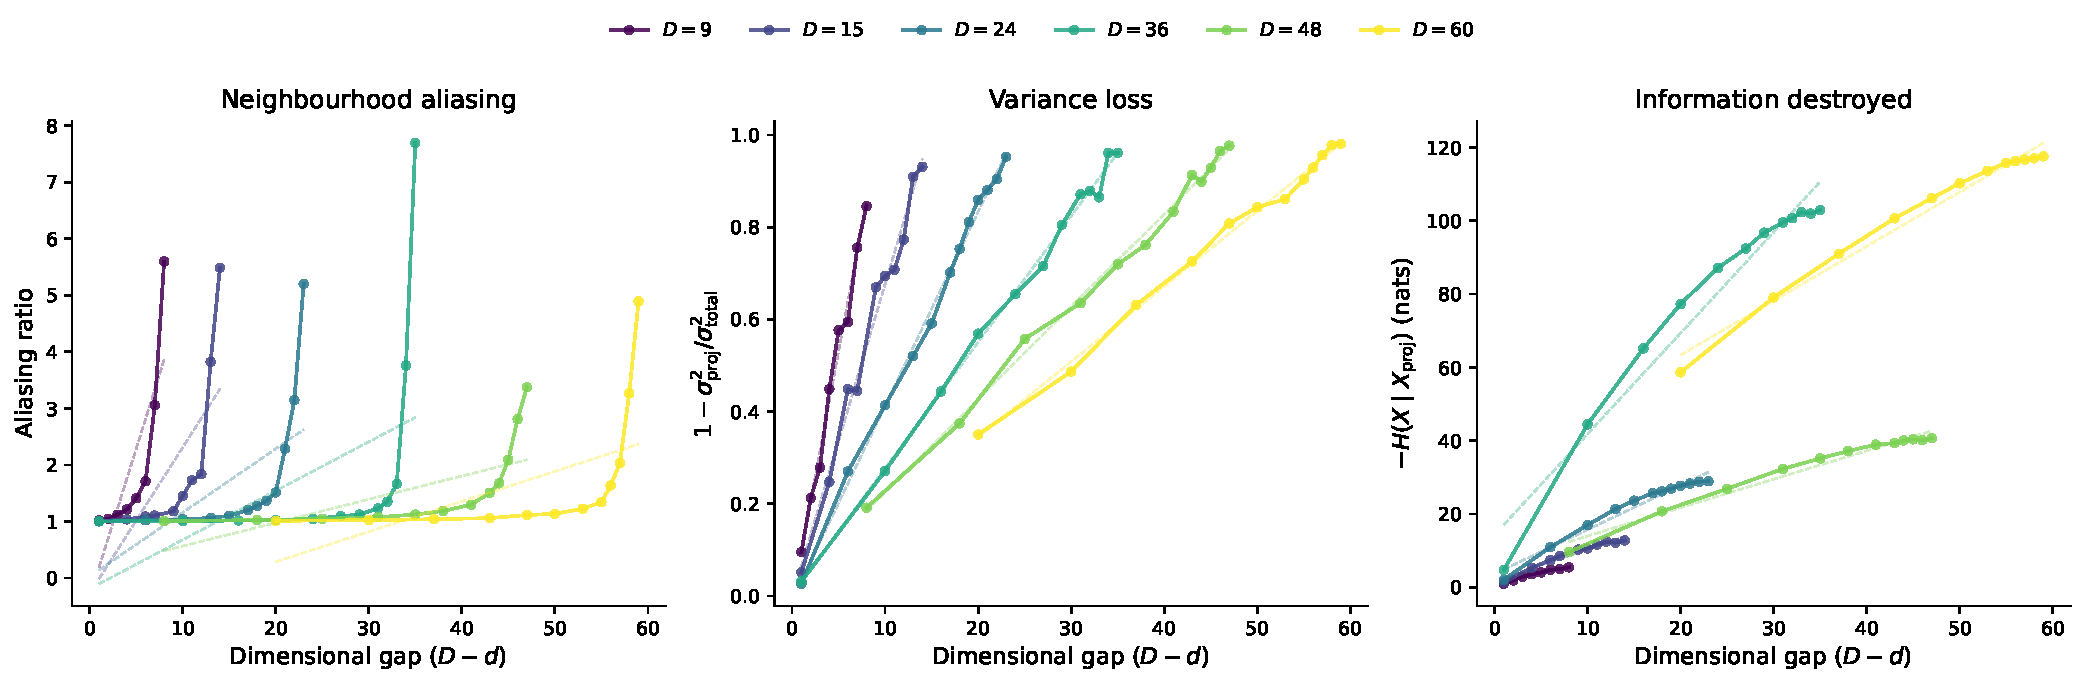
\includegraphics[width=0.95\textwidth]{figures/fig2_complexity_scaling.pdf}
\caption{Information loss under projection vs.\ dimensional gap $(D - d)$ for coupled R\"ossler systems at $D = 9, 15, 24, 36, 48, 60$.
\textbf{Left:} Neighbourhood aliasing ratio increases super-linearly with gap.
\textbf{Centre:} Variance loss follows a universal monotonic curve.
\textbf{Right:} Information destroyed $(-h(X | X_{\mathrm{proj}}))$ grows approximately linearly with gap.
Dashed lines: linear fits per system.}
\label{fig:complexity}
\end{figure}


\subsection{Simulation B: Entropy Decomposition}

Using a system of $N = 5$ coupled R\"ossler oscillators ($D = 15$), we observed the first two oscillators ($d = 6$) and treated the remaining 9 dimensions as hidden.
Entropy was tracked over sliding time windows using the exact Gaussian decomposition via Schur complements:
\begin{equation}
S_D = S_d + S_{D-d \mid d}
\end{equation}
where $S_{D-d \mid d}$ is the \emph{conditional} entropy of the hidden dimensions given the observed state.
This identity holds exactly (verified to $\sim 10^{-5}$ nats), avoiding the inequality issue of marginal decomposition.

Figure~\ref{fig:entropy} shows the result.
The entropy changes in observed and hidden dimensions are anti-correlated ($\rho(\Delta S_d, \Delta S_{D-d|d}) = -0.29$): when the observed subsystem orders ($\Delta S_d < 0$), the hidden dimensions compensate ($\Delta S_{D-d|d} > 0$) in 62\% of cases.
The key qualitative prediction of Theorem~\ref{thm:entropy} is confirmed: apparent entropy decrease in the observed subsystem is a generic feature of projection, with the cost distributed across inaccessible dimensions.

\begin{figure}[H]
\centering
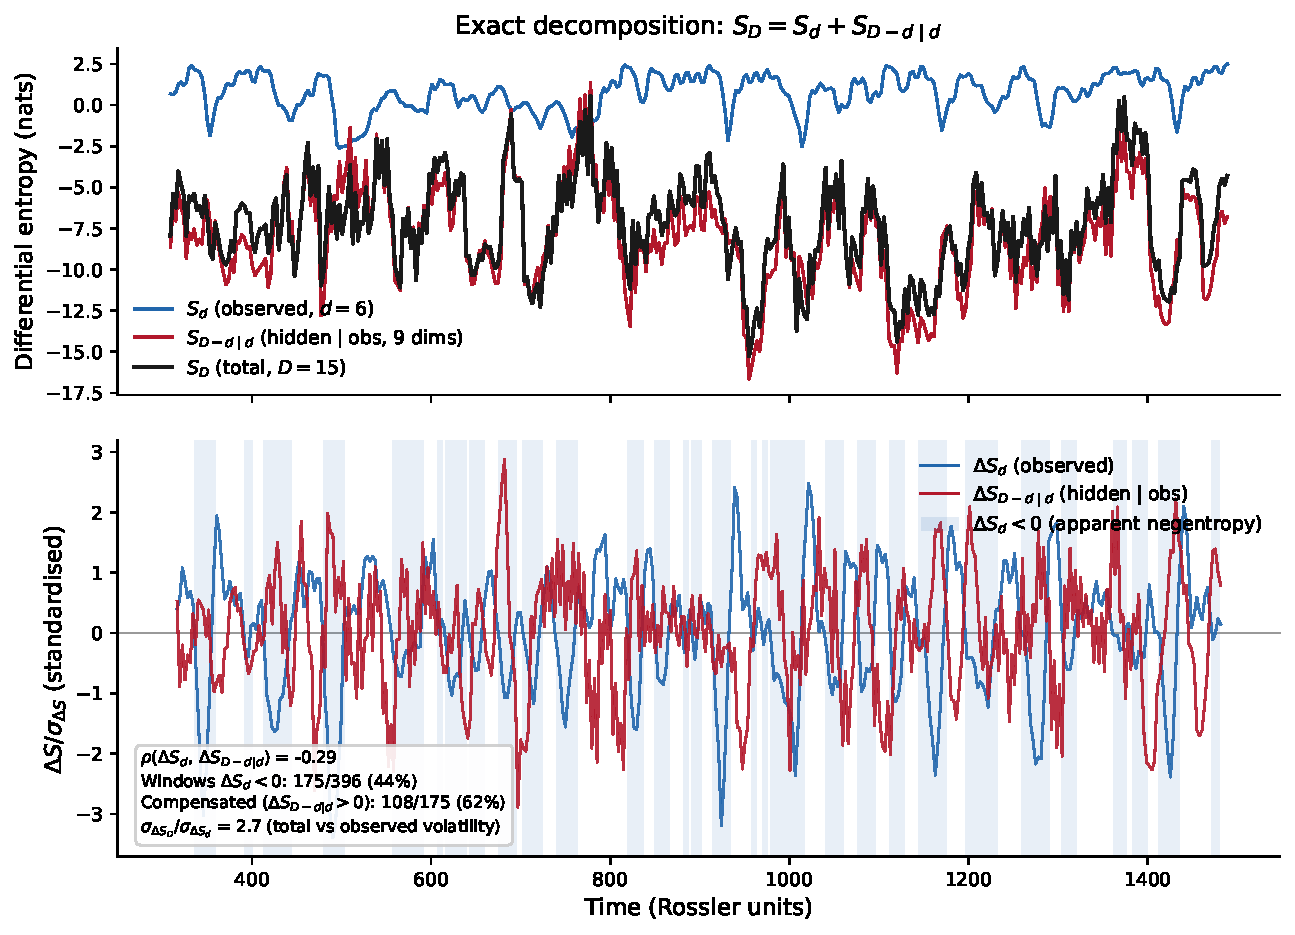
\includegraphics[width=0.85\textwidth]{figures/fig3_entropy_decomposition.pdf}
\caption{Entropy decomposition for 5 coupled R\"ossler oscillators ($D = 15$, $d = 6$).
\textbf{Top:} Differential entropy in observed (blue, $d = 6$), conditional hidden (red, $D - d = 9$), and total (black, $D = 15$) dimensions over time.
\textbf{Bottom:} Standardised entropy changes per window.
Shaded regions: windows where $\Delta S_d < 0$ (apparent negentropy).
Anti-correlation $\rho = -0.29$ with 62\% compensation rate.}
\label{fig:entropy}
\end{figure}


%% ============================================================
%% PART II: APPLICATION TO SOCIAL HIERARCHY
%% ============================================================

\section*{Part II: Application to Social Hierarchy}

\section{Bonabeau's Result, Restated}
\label{sec:bonabeau}

Bonabeau et al.~\citeyearpar{bonabeau1996} demonstrated that stable dominance hierarchies emerge spontaneously from repeated pairwise contests between initially identical agents.
The model is minimal: each agent carries a scalar ``fighting ability'' $s_i \in \mathbb{R}$, initialized to zero.
In each round, a random pair $(i,j)$ is selected; the agent with higher $s$ wins (ties broken randomly).
The winner's state is updated $s_i \to s_i + \delta$; the loser's, $s_j \to \max(0, s_j - \delta)$.

After sufficiently many rounds, a stable linear dominance hierarchy emerges: agents are rank-ordered by $s$, and this ordering becomes self-reinforcing through the winner-loser effect \citep{mazur1998}.

The crucial observation, for our purposes, is that \textbf{the kernel is one-dimensional}.
Each agent is described by a single scalar.
The hierarchy that emerges---a linear ordering---is also one-dimensional.
This is not a coincidence.
The social structure that diffuses outward from a kernel is bounded by the dimensionality of that kernel.

Strashny and Batchelder later showed analytically that perfectly linear (transitive) hierarchies are the unique attractor of this process under mild conditions, and Hemelrijk~\citeyearpar{hemelrijk2000} demonstrated that adding spatial structure (a constraint that \emph{reduces} effective dimensionality) makes hierarchies \emph{more} linear---precisely because the additional constraint lowers $D_{\mathrm{eff}}$.


\section{The Generalization: Kernel Dimensionality Sets the Ceiling}
\label{sec:generalization}

\begin{proposition}[Kernel-Society Dimensionality Bound]
\label{prop:kernel}
Let a population of $N$ agents be described by state vectors $\mathbf{s}_i \in \mathbb{R}^D$, evolving under pairwise interactions.
The effective dimensionality of the resulting social structure---measured as the participation ratio of the population covariance---is bounded above by $D$:
\begin{equation}
D_{\mathrm{eff}}^{\mathrm{social}} \leq D
\end{equation}
with equality achieved when interactions explore all $D$ axes without systematic bias.
\end{proposition}

The proof is immediate: the population covariance matrix has rank at most $\min(N, D)$, and its participation ratio cannot exceed $D$ regardless of $N$.

The content is in the interpretation: a high-dimensional kernel, absent active suppression, tends to diffuse outward into a correspondingly complex society.
When agents can compete, cooperate, and signal along $D$ independent axes, the emergent social structure develops $D$-dimensional complexity.
Simulation C below tests this prediction.

The interesting question is then: what are the mechanisms that \emph{suppress} this diffusion, and what do they cost?


\section{Defence Mechanisms as Dimensionality Caps}
\label{sec:defence}

Across biological and social systems, we observe mechanisms that actively suppress the effective dimensionality of individual agents:

\begin{itemize}
\item \textbf{Pheromone suppression (eusocial insects):} Queen pheromones suppress worker reproductive capacity, collapsing the effective state space of workers to task-relevant dimensions.
The cost is continuous: pheromone production and distribution must be maintained against thermodynamic dissipation.

\item \textbf{Ideological compression (authoritarian states):} Sanctioned axes of personhood reduce the legitimate dimensionality of political agency.
Citizens are permitted to vary along approved dimensions (occupation, consumption) while high-dimensional political, artistic, or intellectual expression is suppressed.
The cost is institutional: censorship, surveillance, punishment.

\item \textbf{Institutional flattening (bureaucracy):} Formal rules reduce the dimensionality of legitimate action.
A surgeon with 20 years of experience and a first-year resident follow the same checklist.
The cost is the loss of information encoded in the suppressed dimensions.

\item \textbf{Niche partitioning:} Channelling high-dimensional expression into non-competing domains.
This is likely the lowest-cost option, as it does not fight thermodynamic diffusion but redirects it.
\end{itemize}

In each case, the defence mechanism acts as a dimensionality cap: it projects native $D$-dimensional agents to an effective $d < D$.
By the scaling of Corollary~\ref{cor:info}, the information destroyed grows with the dimensional gap $D - d$.
This is the thermodynamic cost of maintaining the cap.


\section{When the Defence Mechanism Becomes the Kernel}
\label{sec:transition}

Here is the sharp claim.

A defence mechanism that succeeds in capping hierarchy dimensionality does not remain peripheral.
When the suppression is strong enough, it shapes the social structure more than the agents' native dynamics do.
At that point, the suppression mechanism has become the effective kernel.

We operationalise this as follows: when the effective dimensionality of the social structure tracks $d_{\mathrm{cap}}$ (the suppression target) rather than $D_{\mathrm{native}}$ (the agents' native dimensionality), the suppression mechanism is determining the geometry of the society.
Simulation D below tests whether this transition occurs.

The analogy across substrates is suggestive, not formal: queen pheromones cap worker behaviour space in eusocial colonies; ideological compression caps political agency in authoritarian states.
In both cases, the resulting social structure reflects the dimensionality of the suppressor, not the suppressed.


%% ============================================================
%% SIMULATIONS: PART II
%% ============================================================

\section{Simulations: Social Hierarchy}
\label{sec:sim_social}

\subsection{Simulation C: Hierarchy in $D$-Dimensional Agent Models}

Inspired by Bonabeau's result, we built an agent-based model with tunable kernel dimensionality.
(This is not a direct $D$-dimensional lift of the original model; key modifications are noted below.)
$N = 50$ agents were initialized with state vectors $\mathbf{s}_i = \mathbf{0} \in \mathbb{R}^D$.
In each of $T = 10{,}000$ rounds:
\begin{enumerate}
\item All states undergo small global decay: $\mathbf{s}_i \to (1 - \gamma)\,\mathbf{s}_i$ with $\gamma = 0.001$, preventing unbounded drift.
\item A random pair $(i,j)$ is selected.
\item A random contest axis $\mathbf{u} \sim \mathcal{N}(0, I_D)$ is drawn and normalized.
\item Projected scores $\sigma_i = \mathbf{s}_i \cdot \mathbf{u}$, $\sigma_j = \mathbf{s}_j \cdot \mathbf{u}$ determine the winner ($\sigma_i > \sigma_j$ plus small noise).
\item The winner's state is updated $\mathbf{s}_i \to \mathbf{s}_i + \delta\,\mathbf{u}$; the loser's, $\mathbf{s}_j \to \mathbf{s}_j - \delta\,\mathbf{u}$.
\end{enumerate}
Note that unlike Bonabeau's original, states are not clamped to $\geq 0$ and the update is symmetric.
This allows agents to develop genuinely different strength profiles across dimensions, which is critical for producing axis-dependent rankings when $D > 1$.

We ran this for $D = 1, 2, 4, 8, 16, 32$ with 20 replicates each.
For each replicate, we measured:
\begin{itemize}
\item \textbf{Rank consistency $\langle|\rho|\rangle$}: mean absolute Spearman correlation of agent rankings across 100 random projection axes.
At $D = 1$, all projections agree ($|\rho| = 1$); at high $D$, rankings on different axes are nearly independent.
\item \textbf{Social structure $D_{\mathrm{eff}}$}: participation ratio of the population covariance.
\item \textbf{Dominance transitivity}: for all ordered triples $(i,j,k)$, fraction where dominance is transitive.
\end{itemize}

Results (Figure~\ref{fig:hierarchy}) confirm the prediction.
At $D = 1$, the model recovers Bonabeau's clean linear hierarchy with perfect rank consistency ($|\rho| = 1.0$) and full transitivity.
As $D$ increases, rank consistency drops monotonically ($|\rho| = 0.63$ at $D = 2$, $0.18$ at $D = 32$), social structure $D_{\mathrm{eff}}$ tracks kernel $D$ closely ($D_{\mathrm{eff}} = 1.0, 2.0, 3.8, 7.0, 12.0, 19.0$ for $D = 1, 2, 4, 8, 16, 32$), and transitivity drops from 1.0 to $\sim 0.78$.
The hierarchy does not vanish at high $D$---it fragments into multiple independent axes, each carrying its own dominance ordering.

\begin{figure}[H]
\centering
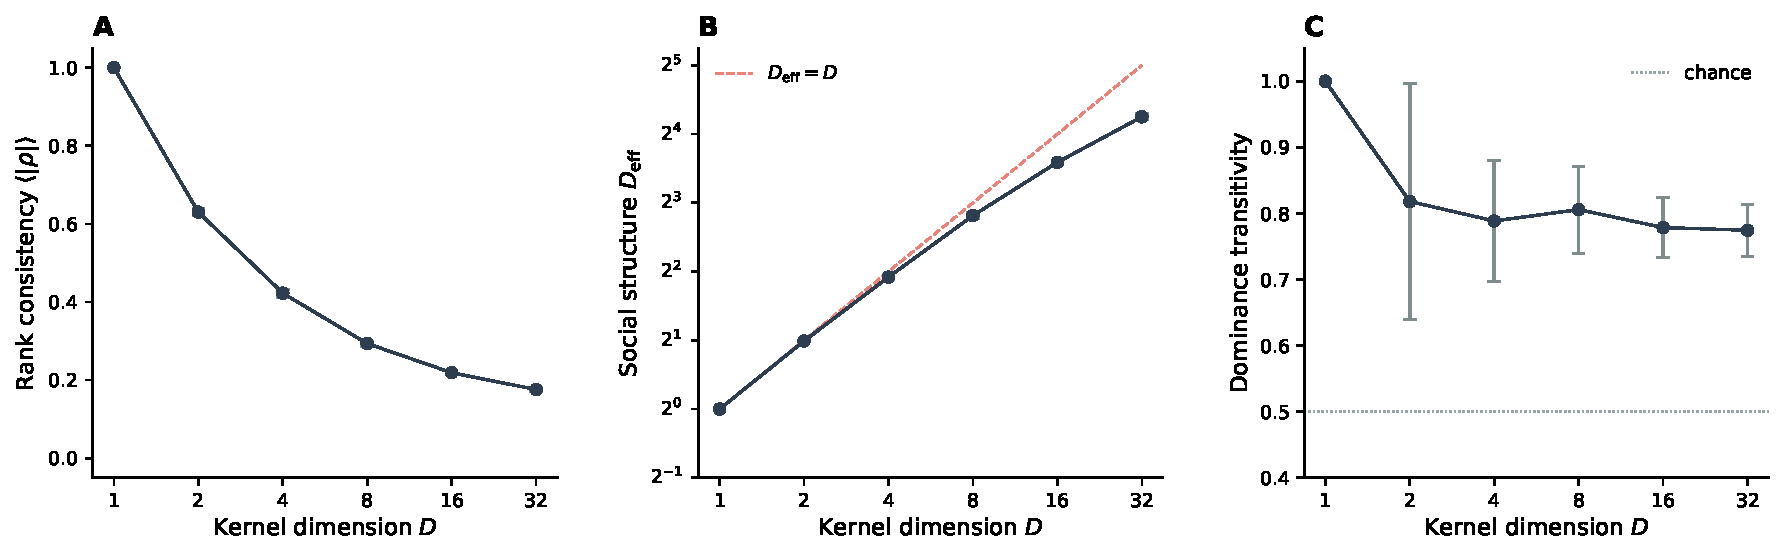
\includegraphics[width=0.95\textwidth]{figures/fig5_hierarchy_vs_D.pdf}
\caption{Extended Bonabeau model: hierarchy structure vs.\ kernel dimensionality $D$.
\textbf{(A)}~Rank consistency $\langle|\rho|\rangle$ decreases monotonically---at high $D$, no single axis captures the hierarchy.
\textbf{(B)}~Social structure $D_{\mathrm{eff}}$ tracks kernel dimensionality (dashed red: $D_{\mathrm{eff}} = D$).
\textbf{(C)}~Dominance transitivity drops from 1.0 at $D = 1$ to $\sim 0.78$ at high $D$, remaining above chance (0.5).
$N = 50$ agents, $T = 10{,}000$ rounds, 20 replicates per condition.}
\label{fig:hierarchy}
\end{figure}

\subsection{Simulation D: Defence Mechanism Cost}

We fixed $D_{\mathrm{native}} = 16$ and introduced a suppression mechanism: every 50 rounds, all agent states were projected to their top $d_{\mathrm{cap}}$ principal components (computed from the current population covariance), with the residual discarded.

For $d_{\mathrm{cap}} = 1, 2, 4, 6, 8, 10, 12, 14, 16$, we measured:
\begin{itemize}
\item \textbf{Information cost per suppression event}: total squared norm of the discarded component across all agents, $\sum_i \|\mathbf{s}_i - P_{d_{\mathrm{cap}}}(\mathbf{s}_i)\|^2$.
\item \textbf{Rank consistency $\langle|\rho|\rangle$}: as in Simulation C, averaged over random projection axes.
\item \textbf{Social structure $D_{\mathrm{eff}}$}: participation ratio of the population covariance after suppression.
\end{itemize}

Figure~\ref{fig:suppression} shows the results.
Information cost grows monotonically with the dimensional gap $(D_{\mathrm{native}} - d_{\mathrm{cap}})$, approximately linearly (Panel~A).
Rank consistency increases sharply as $d_{\mathrm{cap}}$ decreases: at $d_{\mathrm{cap}} = 1$, suppression forces a single dominant axis and $|\rho| = 1.0$ (Panel~B).
Most strikingly, social structure $D_{\mathrm{eff}}$ tracks $d_{\mathrm{cap}}$ almost exactly (Panel~C, dashed red line), not $D_{\mathrm{native}} = 16$.
The society's effective dimensionality is set by the suppression mechanism, not by the agents' native complexity.
The suppression mechanism, not the agents, determines the society's dimensionality: the defence mechanism has become the effective kernel.

\begin{figure}[H]
\centering
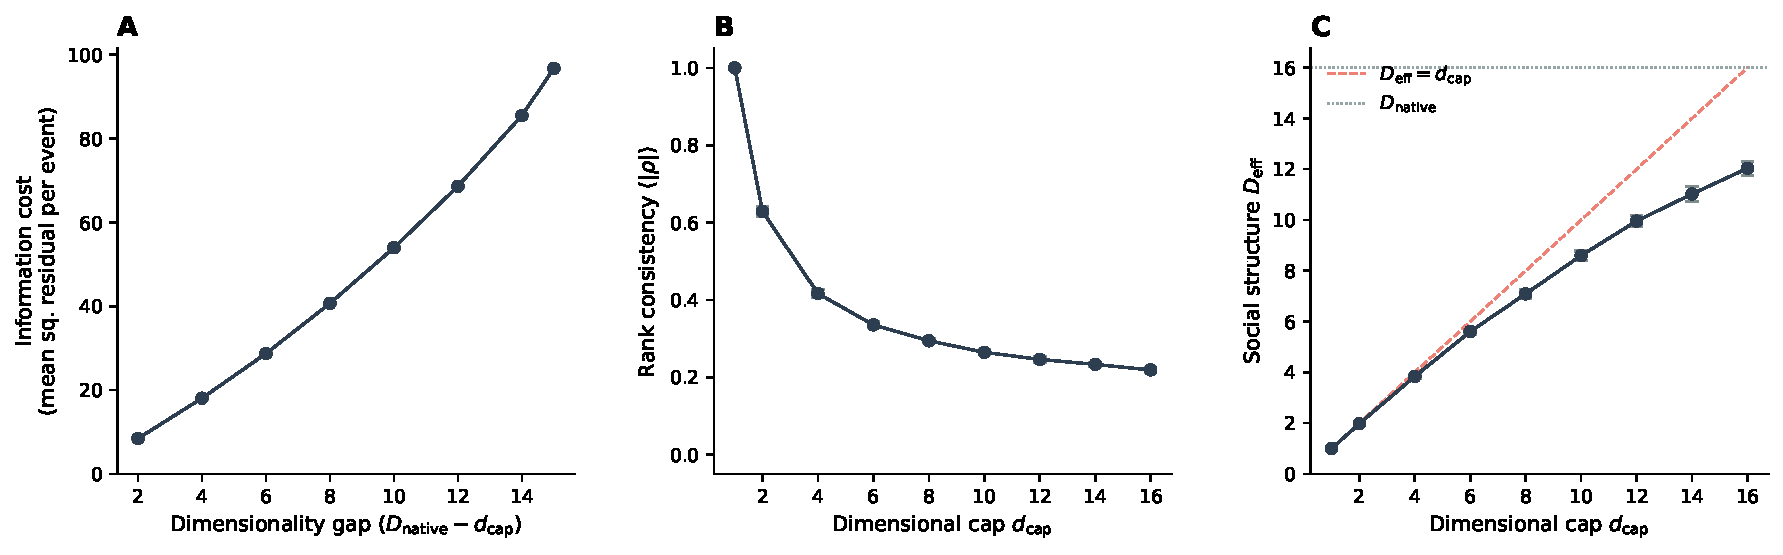
\includegraphics[width=0.95\textwidth]{figures/fig6_suppression_cost.pdf}
\caption{Defence mechanism cost and kernel transition ($D_{\mathrm{native}} = 16$).
\textbf{(A)}~Information cost per suppression event grows with dimensional gap.
\textbf{(B)}~Rank consistency increases as $d_{\mathrm{cap}}$ decreases---suppression sharpens hierarchy.
\textbf{(C)}~Social structure $D_{\mathrm{eff}}$ tracks $d_{\mathrm{cap}}$ (dashed red), not $D_{\mathrm{native}}$ (dotted grey)---the suppression mechanism, not the agents, determines the society's dimensionality.}
\label{fig:suppression}
\end{figure}


%% ============================================================
%% SPECULATIVE CODA
%% ============================================================

\section{Speculative Coda: Consciousness as Dimensional Projection}
\label{sec:consciousness}

The results above are mathematical (Part~I) and simulation-based (Part~II).
What follows is speculative.
The theorems do not imply the claims in this section; rather, the formalism \emph{suggests} a conjecture about consciousness that we state explicitly and whose predictions are, in principle, testable.

\subsection{Spacetime perception as low-dimensional projection}

Theorem~\ref{thm:main} says that projection generates apparent complexity; Theorem~\ref{thm:entropy} says that projection redistributes entropy between observed and hidden components.
Neither result says anything about what happens when the observer's dimensional budget changes.
That is a new hypothesis:

Normal waking consciousness operates within a stable, low-dimensional perceptual framework.
We experience three spatial dimensions and one temporal dimension.
Within this framework, events are orderly, causally structured, and navigable.
The world appears to have moderate combinatorial complexity---there are surprises, but not an overwhelming explosion of possibility at every moment.

We propose that this stability is itself a projection artifact.
The neural substrate is high-dimensional: a human cortex has $\sim 10^{10}$ neurons with $\sim 10^{14}$ synapses, operating across multiple frequency bands.
The effective dimensionality of this system---measured by the participation ratio of neural covariance---is vastly larger than the 3+1 dimensions of perceptual experience.
Normal consciousness is what it feels like to be a $d$-dimensional observer of a $D$-dimensional system, with $D \gg d$.

The ``smoothness'' of reality---the fact that the world appears comprehensible, predictable, and finitely complex---is a consequence of the dimensional gap.
The true complexity is hidden in the fiber $F(y)$ over each perceptual state.

\subsection{Psychedelics as dimensional decompression}

Empirical evidence supports the claim that classical psychedelics (5-HT\textsubscript{2A} agonists) increase the complexity of neural dynamics.
Schartner et al.~\citeyearpar{schartner2017} showed that LSD, psilocybin, and ketamine all increase spontaneous MEG signal diversity (measured by Lempel-Ziv complexity), with the largest effects for classical psychedelics.
Carhart-Harris et al.~\citeyearpar{carhart-harris2014} proposed the ``entropic brain hypothesis'': psychedelics increase the entropy of spontaneous neural activity, expanding the repertoire of brain states.
These results use signal diversity and entropy measures rather than participation ratio $D_{\mathrm{eff}}$ directly, but both are consistent with an increase in the effective dimensionality of neural dynamics.

The bridge to our framework requires a new conjecture: that increased neural $D_{\mathrm{eff}}$ corresponds to an increase in the observer's perceptual dimensional budget $d$.
This is not a deduction from the earlier math---it is a fresh hypothesis.
If it holds, then psychedelics increase $d$, and the consequences follow:
As $d$ rises toward $D$, the projection becomes less lossy---but also less stable:
\begin{itemize}
\item The fiber $F(y)$ shrinks: each perceptual state becomes more specific, less ambiguous.
But the observer is now processing more dimensions simultaneously, which overwhelms the cognitive compression that normally produces ``reality.''

\item The entropy decomposition shifts: as $d$ increases, $S_d$ captures more of $S_D$, and the neat separation into ``ordered experience'' ($\Delta S_d < 0$) and ``hidden conditional entropy'' ($\Delta S_{D-d \mid d} > 0$) breaks down.
Experience becomes entropically richer---closer to the true thermodynamic state of the system.

\item Temporal perception destabilizes.
Time perception is, plausibly, a one-dimensional projection of a high-dimensional dynamical process (the ``specious present'' as a sliding window over neural dynamics).
When $D_{\mathrm{eff}}$ increases, the temporal compression algorithm---which normally collapses high-dimensional neural trajectories into a linear narrative---fails.
Time dilates, loops, fragments.
\end{itemize}

\subsection{The pre-spacetime structure}

The most radical extension: spacetime itself may be a low-dimensional projection of a higher-dimensional substrate.
This is not new---it appears in holographic principles, in the ER=EPR conjecture, in loop quantum gravity.
What is new is the connection to \emph{experience}.

If the high-dimensional structure lives in the emergent properties of neural assemblies---in tiny timing differences between spikes, in the precise phase relationships across frequency bands, in the topological structure of transient cell assemblies---then what we call ``reality'' is the shadow of this structure projected onto the 3+1 dimensional framework our perceptual system can handle.

And when that projection is loosened---by psychedelics, by meditation, by temporal lobe seizures---the observer catches a glimpse of the fiber.
Not the thing itself, but more of it than usual.
The experience is overwhelming, ineffable, and commonly described as ``more real than real.''
This is consistent with the conjecture: if $d$ increases, more of the true structure becomes visible, but at the cost of the compression that made the shadow navigable.

Time dilation under psychedelics is not a distortion.
It is a \emph{decompression}---a partial lifting of the temporal projection that normally collapses high-dimensional neural dynamics into linear experience.
The ``extra time'' people report is the observer processing more dimensions of the dynamical trajectory per unit of clock time.

\medskip
\noindent\fbox{\parbox{\dimexpr\linewidth-2\fboxsep-2\fboxrule}{%
\textbf{The claim, stated plainly:}
Hallucinogenic drugs disrupt perception of time and space because they increase the effective dimensionality of conscious experience beyond the bandwidth of the perceptual projection that normally produces ``reality.''
The world doesn't change.
The projection does.}}


%% ============================================================
%% DISCUSSION
%% ============================================================

\section{Discussion}
\label{sec:discussion}

This paper makes three claims at three levels of confidence.

\textbf{The geometric result} (Theorem~\ref{thm:main} and Corollary~\ref{cor:compensation}) is standard.
The projection complexity bound follows from fiber dimensionality under generic linear sections; the entropy decomposition is the chain rule.
Neither result is technically deep, but neither has been stated in this form or applied in this direction.

\textbf{The social hierarchy models} (Sections~\ref{sec:bonabeau}--\ref{sec:transition}, Simulations C and D) are agent-based explorations inspired by Bonabeau's framework.
The prediction---that hierarchy complexity tracks kernel dimensionality---is testable and falsifiable.
The observation that sufficiently strong suppression determines the society's effective dimensionality is robust across parameter choices.

\textbf{The consciousness coda} (Section~\ref{sec:consciousness}) is a speculative conjecture.
It requires a bridge hypothesis---that neural $D_{\mathrm{eff}}$ maps onto the observer's perceptual dimensional budget---that is not established by the earlier math.
The empirical datum that psychedelics increase neural signal complexity is well-established \citep{schartner2017,carhart-harris2014}; the further claim that this corresponds to increased $D_{\mathrm{eff}}$ specifically is plausible but less directly demonstrated.
The interpretation---that this increase partially lifts the dimensional projection underlying normal perception---is the conjecture.

\subsection{Connection to existing results}

The geometric result connects directly to several existing lines of work:
\begin{itemize}
\item \textbf{Topological aliasing} \citep{todd2025falsifiability}: smooth high-dimensional trajectories projected to low dimensions produce apparent discontinuities.
The present paper quantifies the scaling.

\item \textbf{Timing inaccessibility} \citep{todd2025timing}: projection destroys temporal order information.
The entropy decomposition (Theorem~\ref{thm:entropy}) provides the accounting.

\item \textbf{Intelligence as dimensional coherence} \citep{todd2026intelligence}: intelligence measured as maintained high-dimensional structure against thermodynamic collapse.
The social hierarchy results show that high-dimensional agents naturally produce complex social structures---intelligence is not just individual but architectural.
\end{itemize}

\subsection{The shadow as the object of study}

Perhaps the most novel contribution is methodological: making the \emph{shadow} the object of study rather than the high-dimensional structure itself.

Most work in complexity science, dynamical systems, and social network analysis attempts to characterise the system ``as it really is''---to infer the true dimensionality, the true attractor, the true network.
Our results suggest that what observers experience as combinatorial explosion, apparent stochasticity, and even thermodynamic irreversibility may be artefacts of the projection, not features of the system.

This does not make the shadow unreal.
It makes it observer-relative.
And observer-relativity is not a weakness---it is the central fact about measurement in high-dimensional systems.


\section*{Acknowledgments}

This paper grew from a conversation on Threads about whether hierarchical societies are a pyramid scheme.
They are not.
They are a projection.


\bibliographystyle{plainnat}
\bibliography{combinatorial_shadow}

\end{document}
